\section{Starting cold}
\label{sec:cold}

The \emph{cold start problem} has long been known to be a key difficulty in building effective classifiers quickly and cheaply via active learning~\cite{zhuDensity2008, donmez07dual}. Since the quality of data
selection directly depends on the understanding of the space provided by the ``current'' model, early stages of acquisitions can result in a vicious cycle of uninformative selections, leading to poor quality models and therefore additional poor selections.

The difficulties posed by the cold start problem can be particularly acute in highly skewed or disjunctive problem spaces; informative instances may be difficult for active learning to find due to their variety or rarity, potentially leading to substantial waste in data selection.
Difficulties early in the active learning process can, at least in part, be attributed to the base classifier's poor understanding of the problem space. This cold start problem is particularly acute in otherwise difficult domains. Since the value of subsequent label selections depends on base learner's understanding of the problem space, poor selections in the early phases of active learning propagate their harm across the learning curve.

In many research papers active learning experiments are ``primed'' with a preselected, often class-balanced training set.  As pointed out by~\cite{attprovkdd2010} if the possibility and procedure exists to procure a class-balanced training set to start the process, maybe the most cost-effective model-development alternative is not to do active learning at all, but to just continue using this procedure. This is exemplified in Figure~\ref{fig:guidedvary_skew}~\cite{attprovkdd2010},
where the red lines show the effect of investing resources to continue to procure a class-balanced, but otherwise random,
training set (as compared
with the active acquisition shown in Figure~\ref{fig:vary_skew}).

\begin{figure*}[t!]
\center{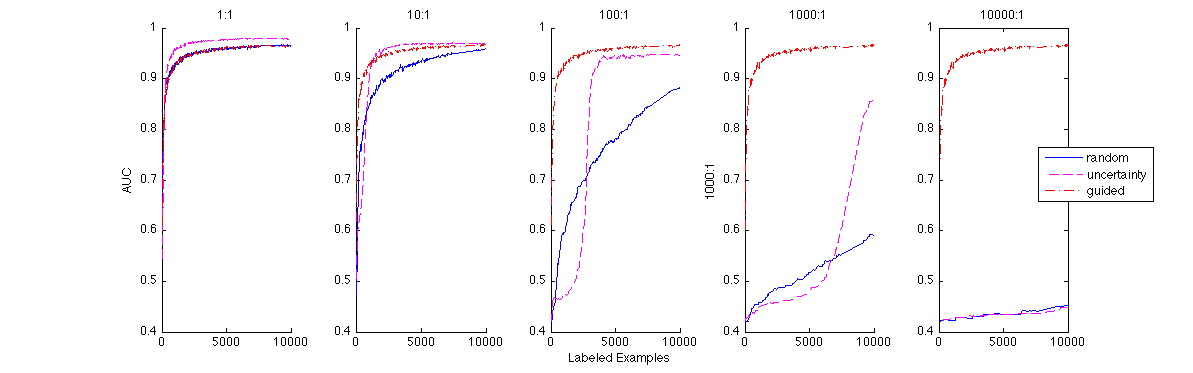
\includegraphics[width=\columnwidth]{plots/varySkewRandUncGuid2.png}}
\caption{Comparison of random sampling and uncertainty sampling and guided learning on the problem seen in Figure~\ref{fig:vary_skew}.}
\label{fig:guidedvary_skew}
\end{figure*}

